\section{The Action}

\ldots

\subsection{Disposition of Forces}

\ldots

\subsection{Opening moves}

\subsubsection{Americans:}

\begin{figure}[h]
    \begin{center}
    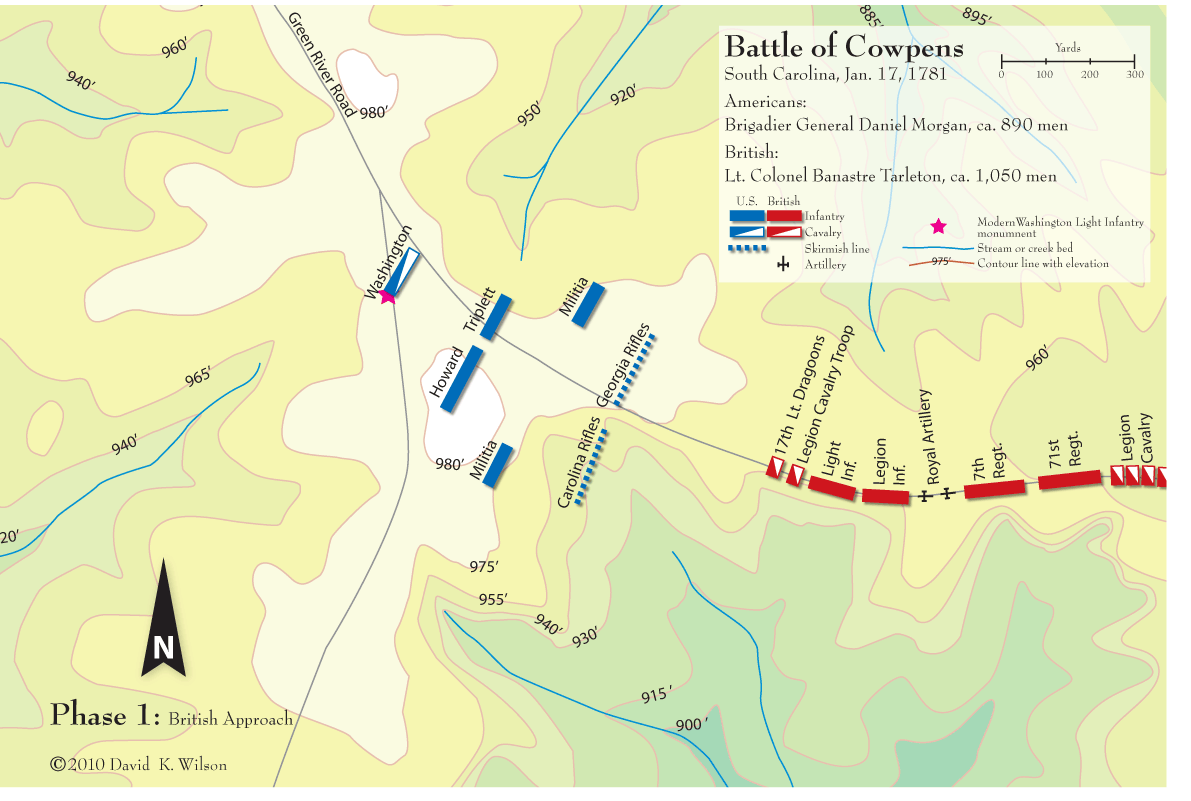
\includegraphics[width=\textwidth]{gfx/beiber01}
    \end{center}
    \caption{Initial disposition of the Armies.\cite{wilson_blogmap}}
    \label{terrain1}
\end{figure}
%\url{http://www.davidwilsonhome.com/homepage/Perspectives/Entries/2010/4/11_The_Battle_of_Cowpens__A_Cartographic_Interpretation.html}

Brigadier General Danial Morgan, knowing that Tarleton was in full pursuit,
selected Cowpens as the field of battle. He describes his decision to fight at
there in later correspondence with Nathanael Greene, ``I would not have had a
swamp in the view of my militia on any consideration; they would have made for
it, and nothing could ha ve detained them from it. As to covering my wings, I
knew my adversary and was perfectly sure I should have nothing but downright
fighting. As to retreat, it was the very thing I wished to cut off all hope of.''
\cite[46]{moncure_cowpens_1996} Morgan had chosen the location for battle and anticipated
Tarleton's forces the following day. He had deployed reconnaissance forces who
would alert him when Tarleton approached and, knowing his men, used the hours
awaiting word of Tarleton's advance to align his forces.

Morgan had selected the time and place for battle. As a result, he took full
use of this advantage over Tarleton in the night prior to the British advance,

\begin{quote}
  ``The night gave Morgan time to prepare his men for combat the next day, and
  the skilled leader made the most of his opportunity. Allowing his troops to
  prepare physically -- cleaning their weapons, eating and so forth -- he walked
  among them to prepare them emotionally for the horrors of eighteenth-century
  battle. Major Thomas Young of South Carolina wrote that Morgan showed a keen
  sense of how to command militia: `He went among the volunteers, helped them
  fix their swords, joked with them about their sweet-hearts, told them to keep
  in good spirits, and the hour would be ours'\,'' \cite[47]{moncure_cowpens_1996}
\end{quote}

After spending the evening resting, rallying, and prepping the troops, Morgan
spent the early morning hours to brief his plan. There is some discrepancy in
reports as to whether Morgan briefed his entire force or just key leadership,
but the fact remains that Morgan competed the task of briefing his plan to
subordinates in sufficient time and fashion to disseminate this information to
his entire force. The task of occupying the defensive line was completed in the
early morning hours before light. Few specific recollections exists regarding
the formal occupation of the American defensive lines, but this action most
likely occurred after the troops had been fully briefed. Once the defense was
established, Morgan and his subordinate leaders spent their time continually
speaking with and rallying the troops.

Morgan was well aware of Tarleton's history, personality, and reputation as an
aggressive combatant. His developed understanding of Tarleton's rash
personality and fierceness in combat led him to make assumptions regarding
Tarleton's actions. Morgan used this knowledge of the British leader and
coupled it with his significant understanding of the troops under his own
command. The result of this analysis was Morgan's choice of defense in order to
attempt to forceTarleton to act impulsively on the battlefield. Morgan also had
an understanding of his own troops and that the Militia were relatively
untrained for combat and nervous facing such impressive formal force. He took
advantage of this knowledge and created a defense which would empower his
inexperienced troops and coerce Tarleton into deploying his forces in a
non-advantageous sequence. By the time Tarleton arrived on the field of battle,
Morgan and his troops were ready and waiting. Morgan's leadership and strong
command and control of the situation had resulted in a force which was ready
for the fight and who possessed great confidence in their leadership.

\subsubsection{British:}

On the morning of 17 January, at approximately three o'clock, Tarleton gave his
troops the order to advance. Having pinpointed the American's location, and
under the belief that they were in full retreat, it was Tarleton's intent to
make the roughly six mile movement and attack the Americans at first light.
Tarleton's troops had arrived at this location only five hours earlier. The
troops had very little to eat and were given a small amount of rest prior to
the movement. This ground patrol took Tarleton's troops from their location at
Morgan's previous camp through freezing streams and dense thick brush in the
cold weather. During this movement, the British troops would march up a reverse
slope, out of the thicket, and onto the field of battle. Tarleton describes the
movement in a narrative:

\begin{quotation}
 ``Three companies of light infantry, supported by the legion infantry, formed
 the advance; the 7th regiment, the guns, and the 1st battalion of the 71st,
 composed the center' and the cavalry and mounted infantry brought up the rear.
 The ground which the Americans had passed being broken, and much intersected
 by creeks and ravines, the march of the British troops during the darkness was
 exceedingly slow, on account of the time employed in examining the front and
 flanks as they proceeded.'' \cite[TAB Q, 14]{rauch_battle_2007}
\end{quotation}

Following the crossing of Thicketty creek, Tarleton released an advanced
reconnaissance party of Cavalry with the express intent of locating Morgan's
defense. The troops rode forward and reported back Morgan's location as well as
an estimate on the size of the American force. Tarleton received this
information and drove forward. There are many accounts by soldiers and
leadership alike which suggests this was not an easy movement. The temperatures
were bitterly cold and, although Morgan's troops had passed through this same
path only a day earlier, there are reports of the British troops attempting to
set fire to the brush in order to blaze a path. Tarleton's troops were on the
hunt, and although they were comprised mainly of seasoned warfighters, it is
likely that the long period of pursuit combined with freezing temperatures, a
short period or rest and preparation, and a difficult movement were having
their effect on the morale and physical readiness of his troops. Babits
describes this movement, ``By all accounts, the British had a difficult time
swimming horses and felling trees for bridges on this exhausting march to
contact. Lieutenant Roderick MacKenzie, traveling with his light infantry
company, may have exaggerated, but crossing knee-deep streams in January is
hard on mind and body.'' \cite[57]{babits_devil_2001}

After approximately four hours of movement, on the frozen morning of January 17,
1781, British Lieutenant Colonel Banistre Tarleton's disciplined group of
British soldiers broke through the woodline at Cowpens to face Brigadier
General Daniel Morgan and his group of Continental army regulars and militia.

Upon breaking through the brush at Cowpens, Tarleton began to organize his
troops. Tarleton's recollection of this instance differs from that of his
troops, ``According to Tarleton, he then directed his line to remove their packs
and to file to the right until the flank force faced its counterpart directly.
Lieutenant Roderick Mackenzie portrays a far more hurried onrush.''
\cite[51]{moncure_cowpens_1996}

Regardless of the time which elapsed while Tarleton prepared his troops for
battle, they were observed by and faced with Morgan's waiting troops. When the
American troops were in sight, Tarleton ordered the British to drop their
excess equipment in order to be lighter for battle. Morgan's troops witnessed
this movement and act of British formal military procedure as the British line
organized and filed itself to the full length of the American Front. The
British troops looked disciplined and impressing as they occupied their assault
positions and the American troops recalled this as an intimidating display.

The movement and rapid occupation of the line were an exercise in British
military protocol. Tarleton's forceful personality had already created
disruption amongst his troops and subordinate leadership. He had maintained a
commanding presence on the battlefield, but lacked either the understanding or
insight necessary to prepare his troops mentally or physically. Instead of
taking the precautions necessary during a deliberate attack, Tarleton's actions
were impulsive. This impulsiveness and rush to battle without taking the
adequate precautions necessary was exactly what Morgan was expecting.

The British had established their line. Tarleton had pressed them forward into
position for battle. The men stood ready to fight, but were likely suffering
from physical exhaustion from little sleep or food. They would meet an
organized force in Morgan's men, who had rested and were prepared for their
attack. Tarleton's forcing of these troops quickly into position to face an
awaiting enemy without staging, attending to priorities of work, or developing
a plan would show from the onset of battle. Tarleton's demanding and forceful
leadership got his troops to the fight and time would tell if it would be
enough to will them to victory. The small psychological advantage Tarleton
gained through the drill and ceremony of his force would soon diminish in the
American's favor with the firing of the battle's first shots.


\begin{figure}[h]
    \begin{center}
    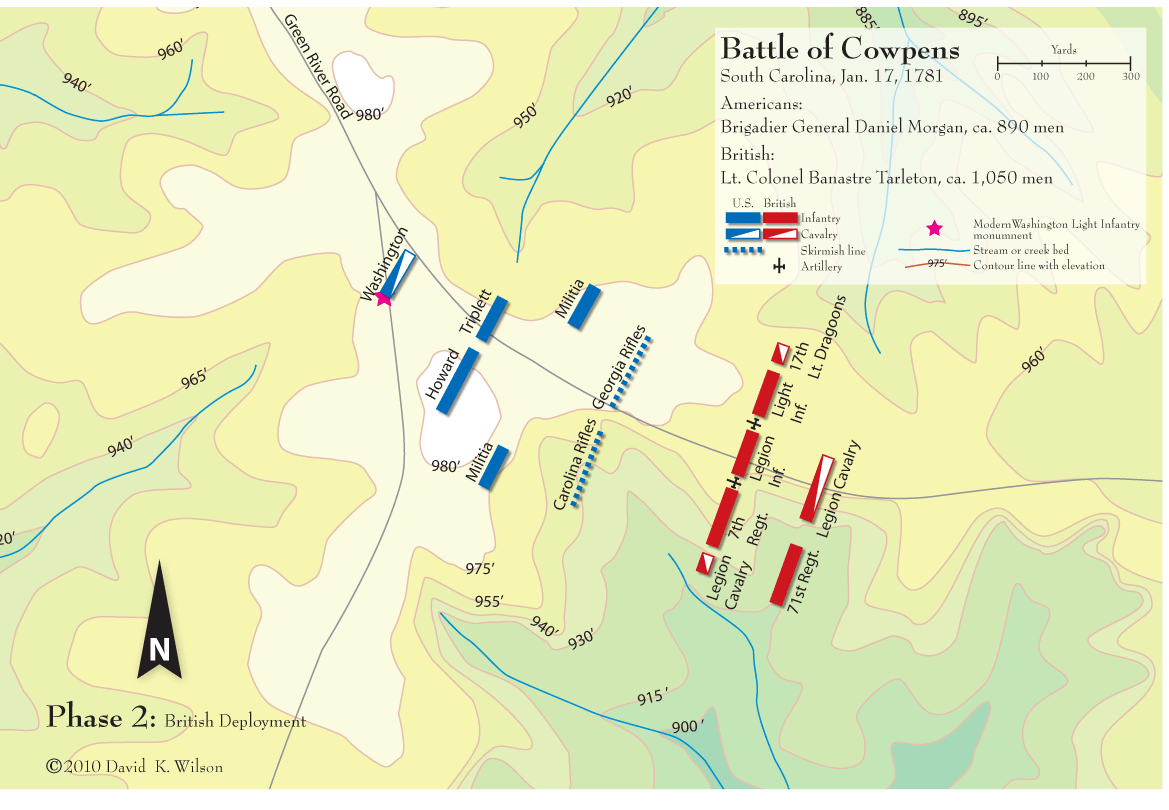
\includegraphics[width=\textwidth]{gfx/beiber02}
    \end{center}
    \caption{British Deployment at the battle of Cowpens \cite{wilson_blogmap}.}
    \label{terrain1}
\end{figure}


\subsubsection{Morgan's Troops Aligned for the Defense}

Brigadier General Morgan had established a three line defense. Morgan's troops
were rested, well briefed, and roused for battle. He had taken full ``home
field'' advantage to use his developed knowledge of the backwoods and
understanding of his troops' abilities to emplace each unit in a role which
suited their strengths. The North Carolina, South Carolina, and Georgia
sharpshooters were out in front, establishing a line of skirmishers intent upon
causing disruption at earliest opportunity. Colonel Andrew Pickens Four
battalions of Virginia militia were next. The third and main line of defense
was the continental Army along with Washington's cavalry held in reserve.

The Sharpshooters from the Southern States were placed approximately 300 meters
in front of the continental line \cite[48]{moncure_cowpens_1996} and only a few
hundred meters in advance of the Virginians. They would be emplaced on an IV
line which would leave Tarleton with little ability to see what lay behind
them. The skirmishers would take cover at this point and begin to engage the
British at earliest opportunity. These men would be tasked to harassment fires
with an intent to disrupt British command and control therefore rushing the
British into a rapid decision making process. These men were by no means meant
to stand and fight.  As soon as the British began an advance or released their
Cavalry in an expected fashion, the skirmishers would fall back and reinforce
the main line of the militia. This would serve another purpose which was the
cornerstone of Morgan's plan: deceive the British into believing the American
lines of defense were breaking down into Retreat.

The Virginia Militia, led by Colonel Andrew Pickens was emplaced at roughly
150m in front of the continental troops' line. These four battalions of men
from the Virginia militia knew their task well and it was with them that the
true battle would begin. Reeling from their assault on the skirmishers, Morgan
assumed the British would organize and attack this line as if it were the main
body. As a result, Morgan emplaced these men behind the skirmishers on level
ground. The militia was tasked with holding their fire until the British came
within less than 100 meters. At that time, they would fire three volleys into
the British line and fall back behind the continental troops led by Lieutenant
Colonel

Howard. This was meant to further exploit the British offensive with aimed
shots at the Officer and Non-Commissioned Officer leadership.

The Delaware and Maryland continental soldiers were led by Lieutenant Colonel
John Eager Howard. Morgan emplaced these troops on slightly elevated terrain.
It was these troops who were tasked with facing and destroying the British
regulars. These troops had seen combat and were prepared for battle. Morgan's
knowledge of the British and of Tarleton specifically led him to this course of
action. It was his intent to cause the British to pursue to the fleeing militia
men so that they met the continental army in an unorganized state with an
overwhelming mass of firepower.

Finally, Morgan placed the 3d Continental Dragoons, led by Lieutenant Colonel
William Washington as a reserve further behind the Continental Troops. This
unit was emplaced out of sight for the British soldiers. Their task was to
reinforce the line and deny the British freedom of maneuver in the event of an
attempted flanking maneuver.

\subsubsection{Tarleton Organizes for Attack}

Tarleton deployed a portion of the Legion Dragoons, on the southeastern flank
of his line. These men were on horseback, and were deployed on the flanks for
maneuverability. These troops were tasked at their location in order to quickly
flank to exploit a weakness or move to deny the Americans freedom of maneuver
on the battlefield. Since these troops were on horseback, they (along with the
17th Dragoons) were the most rested troops in Tarleton's force.

To the right flank of the Dragoons was the 7th Regiment. This unit was deployed
from Britain to the Americas and had seen combat. Their primary task was to
engage and destroy the Americans through firepower and bayonet combat. Since
this was one of the least battle-hardened forces present at Cowpens, Tarleton
likely emplaced these troops in the middle of the line in order to surround
them with security and encourage them to fight.

To the right flank of the 7th Regiment and interspersed in the line were the
men of the Royal Artillery Regiment. Their task was clear, provide direct fire
support and move along with the infantry for security and support.

Next, Tarleton emplaced the Legion Infantry, followed by the light infantry
troops. This further expanding his long line of ground fighters and together
they posed an impressive view of an 18th century force.

Tarleton emplaced the 71st Highlanders in reserve located behind the Legion
Dragoons and 7th Regiment. The intent of this emplacement was likely based upon
necessity rather than preference, ``Tarleton initially desired the 71st to take
position beyond the 7th, but without adequate space to form, the 71st disrupted
the 7th and was then detailed as a reserve.'' \cite[84]{babits_devil_2001}. These men were
battle seasoned and created in Britain strictly for combat in the Americas.
These troops had seen a great deal of combat and were highly regarded in the
Americas as a formidable force.

Finally, the remaining Legion Dragoons, along with Tarleton, took their place
in the rear of the formation for command and control as well as to provide a
reserve force at the immediate control of Tarleton.

\subsection{Action by Phase, and Key Events}

\ldots

\subsection{The Outcome}

\ldots
